% Options for packages loaded elsewhere
% Options for packages loaded elsewhere
\PassOptionsToPackage{unicode}{hyperref}
\PassOptionsToPackage{hyphens}{url}
\PassOptionsToPackage{dvipsnames,svgnames,x11names}{xcolor}
%
\documentclass[
  letterpaper,
  DIV=11,
  numbers=noendperiod]{scrartcl}
\usepackage{xcolor}
\usepackage[margin=1in]{geometry}
\usepackage{amsmath,amssymb}
\setcounter{secnumdepth}{5}
\usepackage{iftex}
\ifPDFTeX
  \usepackage[T1]{fontenc}
  \usepackage[utf8]{inputenc}
  \usepackage{textcomp} % provide euro and other symbols
\else % if luatex or xetex
  \usepackage{unicode-math} % this also loads fontspec
  \defaultfontfeatures{Scale=MatchLowercase}
  \defaultfontfeatures[\rmfamily]{Ligatures=TeX,Scale=1}
\fi
\usepackage{lmodern}
\ifPDFTeX\else
  % xetex/luatex font selection
\fi
% Use upquote if available, for straight quotes in verbatim environments
\IfFileExists{upquote.sty}{\usepackage{upquote}}{}
\IfFileExists{microtype.sty}{% use microtype if available
  \usepackage[]{microtype}
  \UseMicrotypeSet[protrusion]{basicmath} % disable protrusion for tt fonts
}{}
\makeatletter
\@ifundefined{KOMAClassName}{% if non-KOMA class
  \IfFileExists{parskip.sty}{%
    \usepackage{parskip}
  }{% else
    \setlength{\parindent}{0pt}
    \setlength{\parskip}{6pt plus 2pt minus 1pt}}
}{% if KOMA class
  \KOMAoptions{parskip=half}}
\makeatother
% Make \paragraph and \subparagraph free-standing
\makeatletter
\ifx\paragraph\undefined\else
  \let\oldparagraph\paragraph
  \renewcommand{\paragraph}{
    \@ifstar
      \xxxParagraphStar
      \xxxParagraphNoStar
  }
  \newcommand{\xxxParagraphStar}[1]{\oldparagraph*{#1}\mbox{}}
  \newcommand{\xxxParagraphNoStar}[1]{\oldparagraph{#1}\mbox{}}
\fi
\ifx\subparagraph\undefined\else
  \let\oldsubparagraph\subparagraph
  \renewcommand{\subparagraph}{
    \@ifstar
      \xxxSubParagraphStar
      \xxxSubParagraphNoStar
  }
  \newcommand{\xxxSubParagraphStar}[1]{\oldsubparagraph*{#1}\mbox{}}
  \newcommand{\xxxSubParagraphNoStar}[1]{\oldsubparagraph{#1}\mbox{}}
\fi
\makeatother


\usepackage{longtable,booktabs,array}
\newcounter{none} % for unnumbered tables
\usepackage{calc} % for calculating minipage widths
% Correct order of tables after \paragraph or \subparagraph
\usepackage{etoolbox}
\makeatletter
\patchcmd\longtable{\par}{\if@noskipsec\mbox{}\fi\par}{}{}
\makeatother
% Allow footnotes in longtable head/foot
\IfFileExists{footnotehyper.sty}{\usepackage{footnotehyper}}{\usepackage{footnote}}
\makesavenoteenv{longtable}
\usepackage{graphicx}
\makeatletter
\newsavebox\pandoc@box
\newcommand*\pandocbounded[1]{% scales image to fit in text height/width
  \sbox\pandoc@box{#1}%
  \Gscale@div\@tempa{\textheight}{\dimexpr\ht\pandoc@box+\dp\pandoc@box\relax}%
  \Gscale@div\@tempb{\linewidth}{\wd\pandoc@box}%
  \ifdim\@tempb\p@<\@tempa\p@\let\@tempa\@tempb\fi% select the smaller of both
  \ifdim\@tempa\p@<\p@\scalebox{\@tempa}{\usebox\pandoc@box}%
  \else\usebox{\pandoc@box}%
  \fi%
}
% Set default figure placement to htbp
\def\fps@figure{htbp}
\makeatother


% definitions for citeproc citations
\NewDocumentCommand\citeproctext{}{}
\NewDocumentCommand\citeproc{mm}{%
  \begingroup\def\citeproctext{#2}\cite{#1}\endgroup}
\makeatletter
 % allow citations to break across lines
 \let\@cite@ofmt\@firstofone
 % avoid brackets around text for \cite:
 \def\@biblabel#1{}
 \def\@cite#1#2{{#1\if@tempswa , #2\fi}}
\makeatother
\newlength{\cslhangindent}
\setlength{\cslhangindent}{1.5em}
\newlength{\csllabelwidth}
\setlength{\csllabelwidth}{3em}
\newenvironment{CSLReferences}[2] % #1 hanging-indent, #2 entry-spacing
 {\begin{list}{}{%
  \setlength{\itemindent}{0pt}
  \setlength{\leftmargin}{0pt}
  \setlength{\parsep}{0pt}
  % turn on hanging indent if param 1 is 1
  \ifodd #1
   \setlength{\leftmargin}{\cslhangindent}
   \setlength{\itemindent}{-1\cslhangindent}
  \fi
  % set entry spacing
  \setlength{\itemsep}{#2\baselineskip}}}
 {\end{list}}
\usepackage{calc}
\newcommand{\CSLBlock}[1]{\hfill\break\parbox[t]{\linewidth}{\strut\ignorespaces#1\strut}}
\newcommand{\CSLLeftMargin}[1]{\parbox[t]{\csllabelwidth}{\strut#1\strut}}
\newcommand{\CSLRightInline}[1]{\parbox[t]{\linewidth - \csllabelwidth}{\strut#1\strut}}
\newcommand{\CSLIndent}[1]{\hspace{\cslhangindent}#1}



\setlength{\emergencystretch}{3em} % prevent overfull lines

\providecommand{\tightlist}{%
  \setlength{\itemsep}{0pt}\setlength{\parskip}{0pt}}



 


\usepackage{booktabs}
\usepackage{longtable}
\usepackage{array}
\usepackage{multirow}
\usepackage{wrapfig}
\usepackage{float}
\usepackage{colortbl}
\usepackage{pdflscape}
\usepackage{tabu}
\usepackage{threeparttable}
\usepackage{threeparttablex}
\usepackage[normalem]{ulem}
\usepackage{makecell}
\usepackage{xcolor}
\usepackage{placeins}
\usepackage{float}
\KOMAoption{captions}{tableheading}
\makeatletter
\@ifpackageloaded{caption}{}{\usepackage{caption}}
\AtBeginDocument{%
\ifdefined\contentsname
  \renewcommand*\contentsname{Table of contents}
\else
  \newcommand\contentsname{Table of contents}
\fi
\ifdefined\listfigurename
  \renewcommand*\listfigurename{List of Figures}
\else
  \newcommand\listfigurename{List of Figures}
\fi
\ifdefined\listtablename
  \renewcommand*\listtablename{List of Tables}
\else
  \newcommand\listtablename{List of Tables}
\fi
\ifdefined\figurename
  \renewcommand*\figurename{Figure}
\else
  \newcommand\figurename{Figure}
\fi
\ifdefined\tablename
  \renewcommand*\tablename{Table}
\else
  \newcommand\tablename{Table}
\fi
}
\@ifpackageloaded{float}{}{\usepackage{float}}
\floatstyle{ruled}
\@ifundefined{c@chapter}{\newfloat{codelisting}{h}{lop}}{\newfloat{codelisting}{h}{lop}[chapter]}
\floatname{codelisting}{Listing}
\newcommand*\listoflistings{\listof{codelisting}{List of Listings}}
\makeatother
\makeatletter
\makeatother
\makeatletter
\@ifpackageloaded{caption}{}{\usepackage{caption}}
\@ifpackageloaded{subcaption}{}{\usepackage{subcaption}}
\makeatother
\usepackage{bookmark}
\IfFileExists{xurl.sty}{\usepackage{xurl}}{} % add URL line breaks if available
\urlstyle{same}
\hypersetup{
  pdftitle={Banff National Park Activity Trends},
  pdfauthor={Camila Hurtado; Martin Hinojosa},
  colorlinks=true,
  linkcolor={blue},
  filecolor={Maroon},
  citecolor={Blue},
  urlcolor={Blue},
  pdfcreator={LaTeX via pandoc}}


\title{Banff National Park Activity Trends}
\usepackage{etoolbox}
\makeatletter
\providecommand{\subtitle}[1]{% add subtitle to \maketitle
  \apptocmd{\@title}{\par {\large #1 \par}}{}{}
}
\makeatother
\subtitle{Activity Trends 2020-2025}
\author{Camila Hurtado \and Martin Hinojosa}
\date{2026-07-17}
\begin{document}
\maketitle

\clearpage

\renewcommand*\contentsname{Table of contents}
{
\hypersetup{linkcolor=black}
\setcounter{tocdepth}{3}
\tableofcontents
}

\begin{verbatim}
\end{verbatim}

\newpage{}

\section{Land Acknowledgement}\label{land-acknowledgement}

Biodiversity Pathways respectfully acknowledges that our work takes
place on the territories of Treaties 6, 7, 8, and the Métis homeland,
traditional and ancestral lands of First Nations and Métis Peoples,
whose histories, languages, and cultures are directly linked to the
biodiversity that we monitor.

We acknowledge the traditional teachings of the lands that we work on,
and that reciprocal, meaningful, and respectful relationships with
Indigenous peoples make our work possible. We are deeply grateful for
their stewardship of these lands, and we are committed to supporting
Indigenous-led monitoring programs, while learning Indigenous ways of
knowing, being, and doing.

\section{Introduction}\label{introduction}

\subsection{Overview of NABat and the NNW Bat
Hub}\label{overview-of-nabat-and-the-nnw-bat-hub}

North American Bat Monitoring Program (NABat) is a large-scale
coordinated effort to monitor bat species to address gaps in knowledge
and lack of long-term studies across North America (Loeb et al.
2015).The program is administered by the US Geological Survey (USGS) and
implemented by the North by Northwest Bat (NNW) Hub in Alberta, British
Columbia, and S.E Alaska.

NNW Bat Hub was established in 2024 with collaboration from Government
of Alberta, Government of British Columbia, and Government of Alaska.
The hub was formed by combining the previous Alberta Hub and the BC and
southeast Alaska Hub. The implementation of the program within Alberta
has key support from Parks Canada, government of Alberta staff, other
wildlife biologists, Indigenous Nations, community members and
naturalists across the province.

\subsubsection{NABat Monitoring in Banff National
Park}\label{nabat-monitoring-in-banff-national-park}

Banff National Park has been conducting NABat monitoring within one
NABat grid cell (Grid Cell ID: 148842) since 2020. Monitoring efforts
include three long-term stationary sites and a driving transect. In
addition, 10 supplementary sites were surveyed in 2022 and 2023 to
develop a bat species inventory for the park. All data from 2020 to 2023
were processed using automated identification software. In 2024 and 2025
a subset of the data were also manually verified following the
established NABat protocols ((Reichert et al. 2018a)).

\subsection{Threats to bat populations in
Alberta}\label{threats-to-bat-populations-in-alberta}

Bat populations in Alberta face a wide range of threats including
forestry practices, anthropogenic expansion, and climate change among
others. Of these threats, White-Nose Syndrome and wind energy
development have emerged as two of the highest-priority concerns.

\subsubsection{White-Nose Syndrome}\label{white-nose-syndrome}

White-Nose Syndrome (WNS) is a deadly fungal disease caused by the
fungus \emph{Pseudogymnoascus destructans} (\emph{Pd}) that affects
hibernating bats. As of 2026, WNS has been confirmed in nine Canadian
provinces including Alberta ( Figure~\ref{fig-WNS}: CWHC-RCSF (2024)).
Since Pd was first confirmed in AB in 2022, the fungus and the ensuing
disease have spread through the province at a rapid pase and has now
been detected at the provinces largest known hibernacula, Cadamun cave
(Wilkinson, pers. comm.) Continued monitoring of populations in AB is
critical as \emph{Pd} and WNS continue to spread throughout the
province.

\begin{figure}

\centering{

\pandocbounded{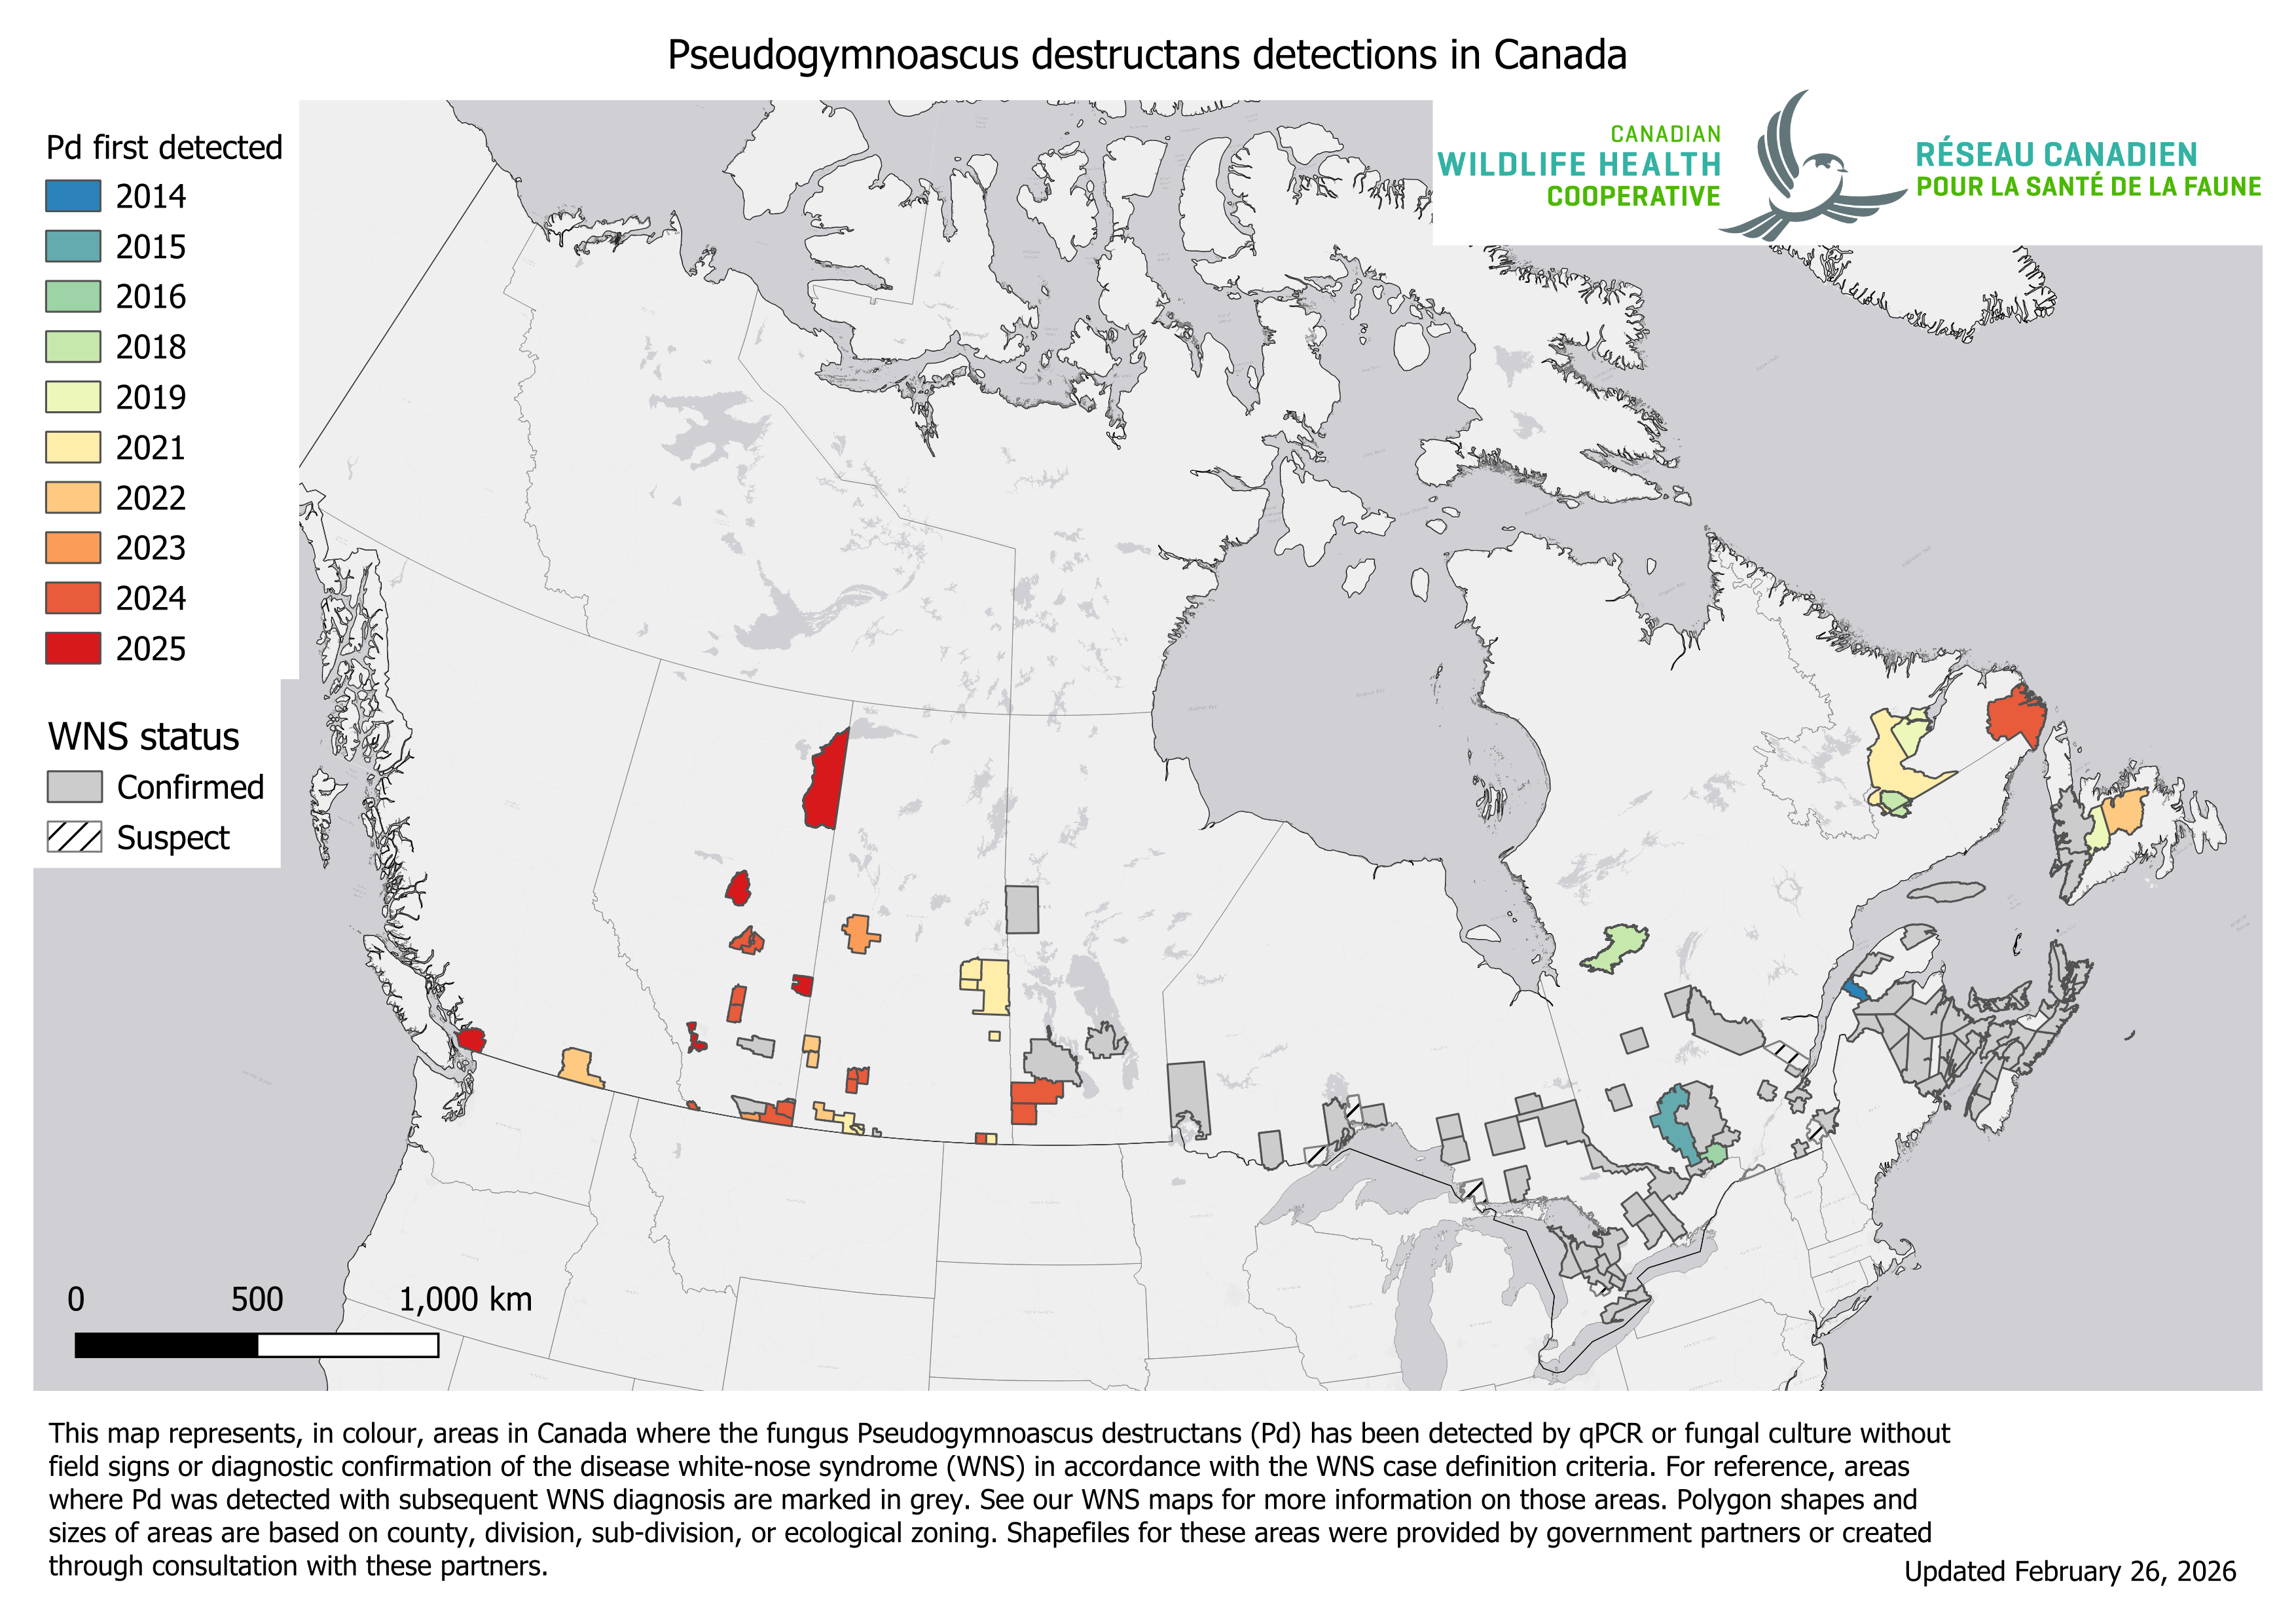
\includegraphics[keepaspectratio]{Figures/Canada-PD.png}}

}

\caption{\label{fig-WNS}White-nose syndrome (WNS) and Pseudogymnoascus
destructans (Pd) occurrence in Canada. Source: CWHC-RCSF (2026)}

\end{figure}%

\subsubsection{Wind Energy Development}\label{wind-energy-development}

Wind energy farms have been linked to high mortality rates across all
bat species in Canada, with long distance migratory species accounting
for 73\% of recorded fatalities (Zimmerling and Francis 2016). In
Alberta alone, one estimate predicts an annual mortality rate 10.9 bats
per turbine (Zimmerling and Francis 2016). There are currently 1,778
turbines active in the province across 49 different projects with the
most turbines found in the grassland ecosystem ({``Canadian Wind Turbine
Database''} (2025) ; Figure~\ref{fig-turbines}). Using Zimmerling and
Francis (2016) estimate, Alberta is estimated to be loosing 19,380 bats
per year to wind turbine collisions. As of 2023, COSEWIC designated all
three of Alberta's long distance migratory species as endangered due in
part to fatalities at wind turbine facilities (Status of Endangered
Wildlife in Canada 2023).

\begin{figure}

\centering{

\pandocbounded{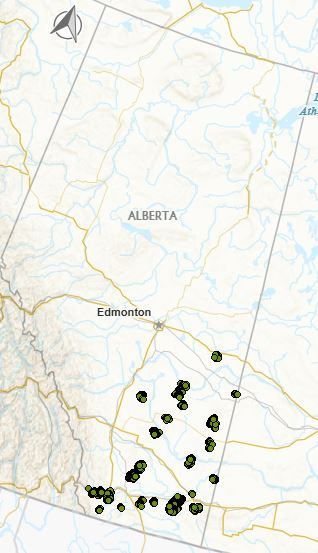
\includegraphics[keepaspectratio]{Figures/AB-Wind.JPG}}

}

\caption{\label{fig-turbines}Current wind turbines in Alberta based on
the Canadian Wind Turbine Database (Source: {``Canadian Wind Turbine
Database''} (2025))}

\end{figure}%

\subsection{Acoustic Monitoring of
Bats}\label{acoustic-monitoring-of-bats}

Acoustic recording is a cost-effective method for monitoring bat
populations across large geographic and temporal scales. However,
several limitations affect the conclusions that can be drawn from these
data:

\begin{enumerate}
\def\labelenumi{\arabic{enumi}.}
\item
  \textbf{Imperfect species identification} --- Bats rely on
  echolocation for hunting and moving around, and species with similar
  ecology and physiology often produce overlapping calls. While
  detectors are deployed to maximize recordings of diagnostic Search
  Phase calls, species identifiability will always vary depending on the
  local species assemblage.
\item
  \textbf{Variable detectability} --- Bat species are not equally
  detectable acoustically. Larger, wide-ranging species produce louder
  calls that travel farther, while smaller species with quieter calls or
  specialized habitat use are less reliably recorded. As a result, trend
  estimates cannot be produced for all species using acoustic methods
  alone.
\item
  \textbf{Data variability} --- Many factors influence recording quality
  and bat activity, including wind speed, humidity, and local habitat.
  Additionally, stationary detectors cannot account for individual
  recapture, meaning acoustic data can only inform relative activity and
  occupancy.
\item
  \textbf{Processing limitations} --- Auto-ID software enables efficient
  processing of large datasets but has known high misclassification
  rates for bats, making manual verification necessary to ensure
  accurate results.
\end{enumerate}

\section{Methods}\label{methods}

\subsection{\texorpdfstring{\emph{Deployments}}{Deployments}}\label{deployments}

\subsubsection{Stationary Surveys}\label{stationary-surveys}

Banff biologists deployed three stationary bat detectors in
strategically selected bat habitat across three distinct quadrants
within the NABat grid cell (Figure~\ref{fig-sites}). These stationary
sites were deployed consistently every year from 2020 to 2025, with
detectors set out between June 24--30 and retrieved between July 2--23 (
Table~\ref{tbl-deployments}). The comparable deployment windows across
years allow for interannual comparison. Deployment setup followed the
standards established by Loeb et al. (2015). Titley Swift units were
used in most years, except in 2020 and 2024, when Wildlife Acoustics SM4
units were deployed instead.

\subsubsection{Transect Surveys}\label{transect-surveys}

The driving transect protocol closely follows that established by Loeb
et al. (2015). Between one and three replicates of a mobile transect
were driven at 30--35 km/h with a bat detector mounted on the vehicle
roof to record bats along the road (Figure~\ref{fig-sites}). Transects
were conducted during the same period that the stationary acoustic units
were deployed (Table~\ref{tbl-deployments}). Titley Walkabout units were
used for all transect deployments across all years.

\begin{table}[H]

\caption{\label{tbl-deployments}Deployments throughout the 6 years of
this monitoring}

\centering{

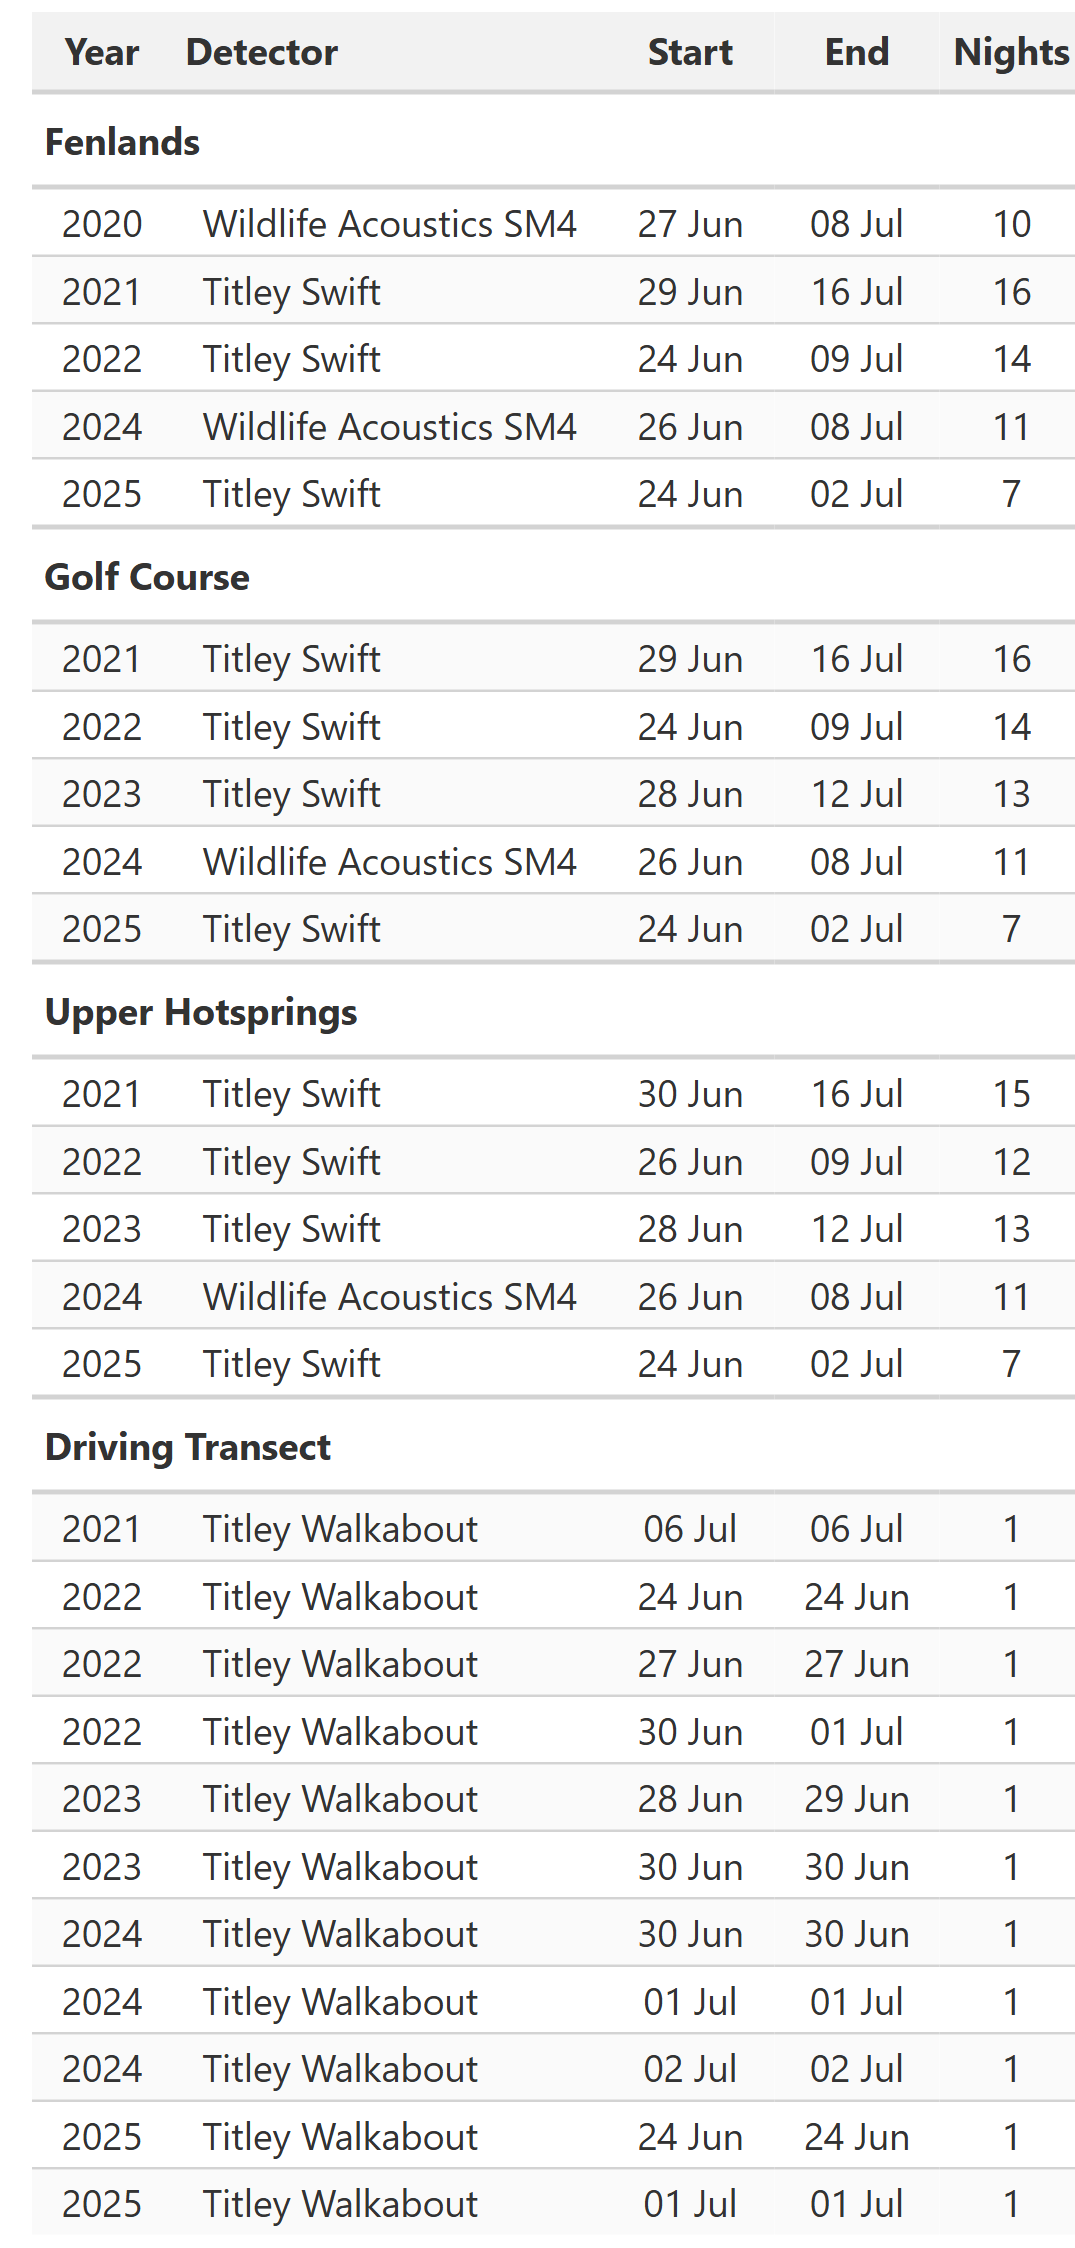
\includegraphics[width=3.58in,height=\textheight,keepaspectratio]{Figures/deploy_table.png}

}

\end{table}%

\subsection{\texorpdfstring{\emph{Manual
Verification}}{Manual Verification}}\label{manual-verification}

All recordings were classified using the Kaleidoscope Pro Bats of North
America 5.4.0 classifier or newer. Automatic classification was used to
assign species identifications and to exclude non-bat recordings. Manual
verification of classifications was conducted for the 2024 and 2025
seasons only, following the processing standards established by the
North American Bat Monitoring Program (NABat) (Reichert et al. 2018b).
Only recordings assigned a species classification by either Kaleidoscope
were selected for manual verification. For stationary acoustic
monitoring, recordings were manually vetted until at least one recording
per species per site per night was confidently identified. For mobile
transects, all recordings with automated species classifications were
manually vetted. Species identifications were validated against
reference call parameters described by Slough et al. (2022), Solick
(2022), and Szewczak (2018), adhering to NABat manual vetting standards
(Reichert et al. 2018b).

Based on documented species ranges and prior detection data (Olson,
n.d.), manual identification efforts focused on seven species: Big Brown
Bats (\emph{Eptesicus fuscus}), Eastern Red Bats (\emph{Lasiurus
borealis}), Silver-haired Bats (\emph{Lasionycteris noctivagans}), Hoary
Bat (\emph{Lasiurus cinereus}), Little Brown Bats (\emph{Myotis
lucifugus}), Long-legged Myotis (\emph{Myotis volans}) and Long-eared
Myotis (\emph{Myotis evotis}).

Trends estimates used only autoID results unless the manual verification
results indicated a bat recordings was actually noise. This was done to
maintain consistency across the 6 years of study, since manual
verification only started in 2024.

All the recordings and results can be found on Widltrax under the Banff
National Park Organization, in the project called
\href{https://portal.wildtrax.ca/aru/3026}{Bat Community - Long Term
Monitoring - NABat - 2020-2025}.

\subsection{\texorpdfstring{\emph{Statistical
Analysis}}{Statistical Analysis}}\label{statistical-analysis}

\subsubsection{\texorpdfstring{\emph{Species
summaries}}{Species summaries}}\label{species-summaries}

Species presence and nightly activity were summarized from a
site--night--species table constructed for all sampled nights. Sampling
effort was defined as the number of unique site-nights on which a
detector was recording. Mean nightly passes include all recordings
assigned a species or couplet label; couplet-labelled files were counted
toward both member species.

\subsubsection{\texorpdfstring{\emph{Environmental
covariates}}{Environmental covariates}}\label{environmental-covariates}

Weather data were obtained from Environment and Climate Change Canada
(ECCC) stations using the \texttt{weathercan} package (Version 1.0.0) in
R and summarized for each sampling night as mean temperature, mean
relative humidity, total precipitation, and mean wind speed. Moon
covariates were calculated for each site-night using the
\texttt{suncalc} package (Version 0.5.1) and included moon illumination
and an index of moon position. All environmental covariates were
standardized (z-scored) prior to modelling to aid convergence and
comparability. The year term was left on its original scale so that
trend estimates represent change per year.

\subsubsection{\texorpdfstring{\emph{Trend
models}}{Trend models}}\label{trend-models}

\paragraph{\texorpdfstring{\textbf{Data
included}}{Data included}}\label{data-included}

Trend models used stationary detector data only. Transect data were not
modelled because the number of recorded call sequences was too low to
support abundance estimation, which requires substantially more sites
(grid cells) and transect replicates than were available here. These
data will nonetheless be useful for modelling species abundance at
provincial or regional scales.

\paragraph{\texorpdfstring{\textbf{Species}}{Species}}\label{species}

Trends were estimated for six taxa: Big Brown Bat (\emph{Eptesicus
fuscus}, EPFU), Eastern Red Bat (\emph{Lasiurus borealis}, LABO), Hoary
Bat (\emph{Lasiurus cinereus}, LACI), Silver-haired Bat
(\emph{Lasionycteris noctivagans}, LANO), Long-eared Myotis
(\emph{Myotis evotis}, MYEV), and a 40 kHz Myotis complex (40KMyo)
comprising \emph{M. lucifugus}, \emph{M. volans}, and \emph{M.
septentrionalis}, whose recordings were summed within each site-night
prior to modelling. Long-eared Myotis is not included in the 40KMyotis
complex due to it's lower frequency call (Fc\textasciitilde30-35kHz).

\paragraph{\texorpdfstring{\textbf{Model structure and
selection}}{Model structure and selection}}\label{model-structure-and-selection}

Nightly bat activity (number of recordings per site-night) was modelled
using negative binomial generalized linear mixed models (GLMMs) with a
log link, fitted in \texttt{glmmTMB} (Version 1.1.12). Each model
included a random intercept for deployment
(\texttt{1\ \textbar{}\ site:year}). This term was used in preference to
a site-only intercept because nights within a deployment share a common
detector, configuration, and weather window, and are therefore not
independent replicates of a year. Fixed effects comprised a linear year
term (years since 2020), a two-level detector-unit term (Wildlife
Acoustics SM4 vs.~Titley Anabat Swift, with Swift as the reference)
included to account for potential differences in detection attributable
to unit type, and a taxon-specific set of environmental covariates.

For each taxon, candidate models were ranked by AICc and the covariate
set from the top-ranked (lowest AICc) model was retained.

\section{Results}\label{results}

Acoustic monitoring happened for a total of 180 detector nights across 3
stationary survey locations and 11 driving transects nights over six
years (2020--2025, Table~\ref{tbl-sppmean}). Survey effort was mostly
even within sites and years with sites sampled for a mean of 12.9 nights
per year (range: 9--17 nights per site-year). A total of 38304 bat
detections were recorded across the three stationary sites and a total
of 475 where collected during driving transects in the Banff NABat grid
cell.

\begin{table}[H]

\caption{\label{tbl-sppmean}Monitoring effort and bat species detections
in the Banff (2020--2025). Mean nightly recordings (± SD) represent
total bat detections per night summed across species. Species detections
indicate presence (X) within each year and quadrant based on combined
automated and manually reviewed identifications. 2024 and 2025 are
bolded to highlight that these were the only years were manual
verification occurred.}

\centering{

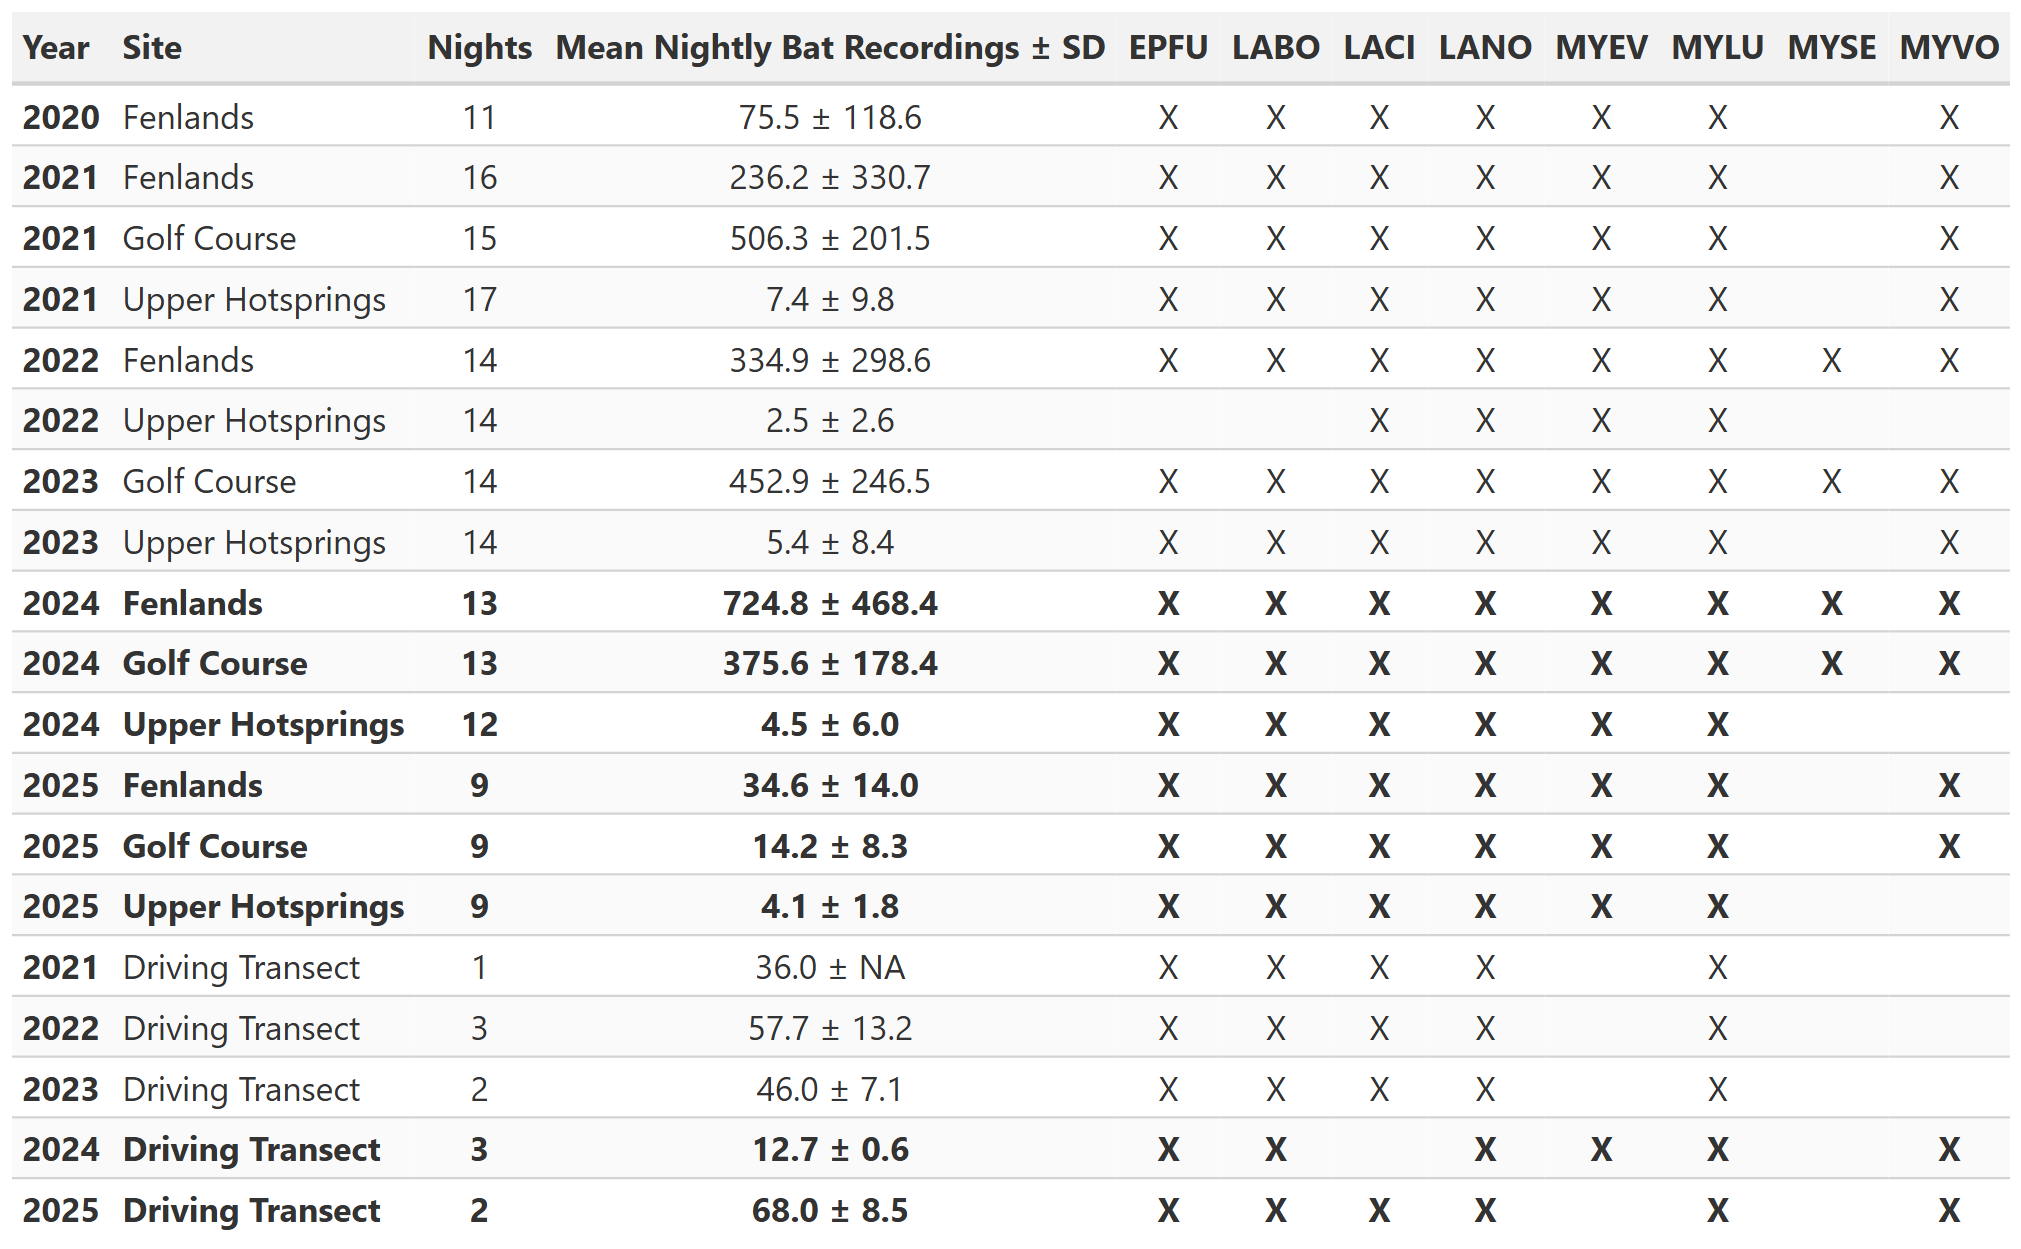
\includegraphics[width=6.74in,height=\textheight,keepaspectratio]{Figures/sppmean_table.png}

}

\end{table}%

\subsection{\texorpdfstring{\emph{Species detected and mean nightly
activity}}{Species detected and mean nightly activity}}\label{species-detected-and-mean-nightly-activity}

Eight species were recorded across the study. Silver-haired bat
(\emph{Lasionycteris noctivagans}) and Little Brown Bat (\emph{Myotis
lucifugus}) were detected across every site and year. Northern myotis
(\emph{Myotis septentrionalis}) was by far the scarcest species,
detected only at Fenlands in 2022 and 2024, and Golf Course in 2023 and
2024 (Table~\ref{tbl-sppmean}, Figure~\ref{fig-sites}). The Little Brown
Bat had the highest number of detections across all years (19617 ;
nightly mean = 102.7068063). This was followed by Long-legged Myotis
(2449 ; nightly mean = 12.8219895), and Eastern Red Bat (1295 ; nightly
mean = 6.7801047).

\begin{figure}[H]

\centering{

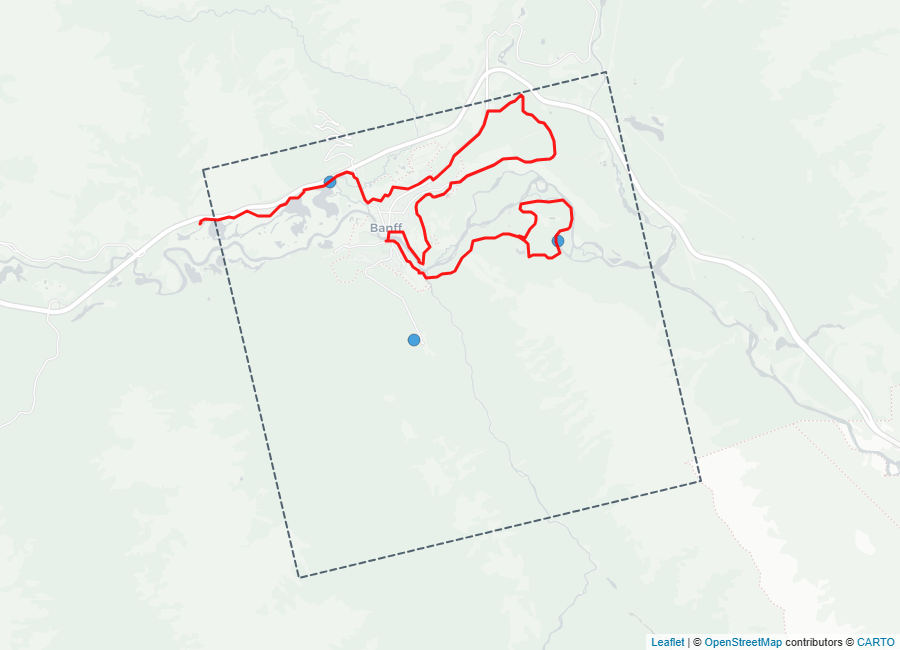
\includegraphics[width=1\linewidth,height=\textheight,keepaspectratio]{Figures/site_summary_map.png}

}

\caption{\label{fig-sites}Acoustic bat monitoring sites in Banff.
Stationary recording stations are shown as blue circular markers and
driving transect is in red line. The boundary of the grid cell is shown
in dashed grey line.}

\end{figure}%

\subsection{\texorpdfstring{\emph{Species
Trends}}{Species Trends}}\label{species-trends}

Models converged for all six species/groups: Big Brown Bat (EPFU),
Eastern Red Bat (LABO), Hoary Bat (LACI), Silver-haired Bat (LANO),
Long-eared Myotis (MYEV) and the combined 40kHz Myotis group (40KMyo)
(Figure~\ref{fig-trends}).

\begin{table}[H]

\caption{\label{tbl-spptrend}Species trend estimate model results. Need
to explain what the estimate is telling us since this is in a log scale}

\centering{

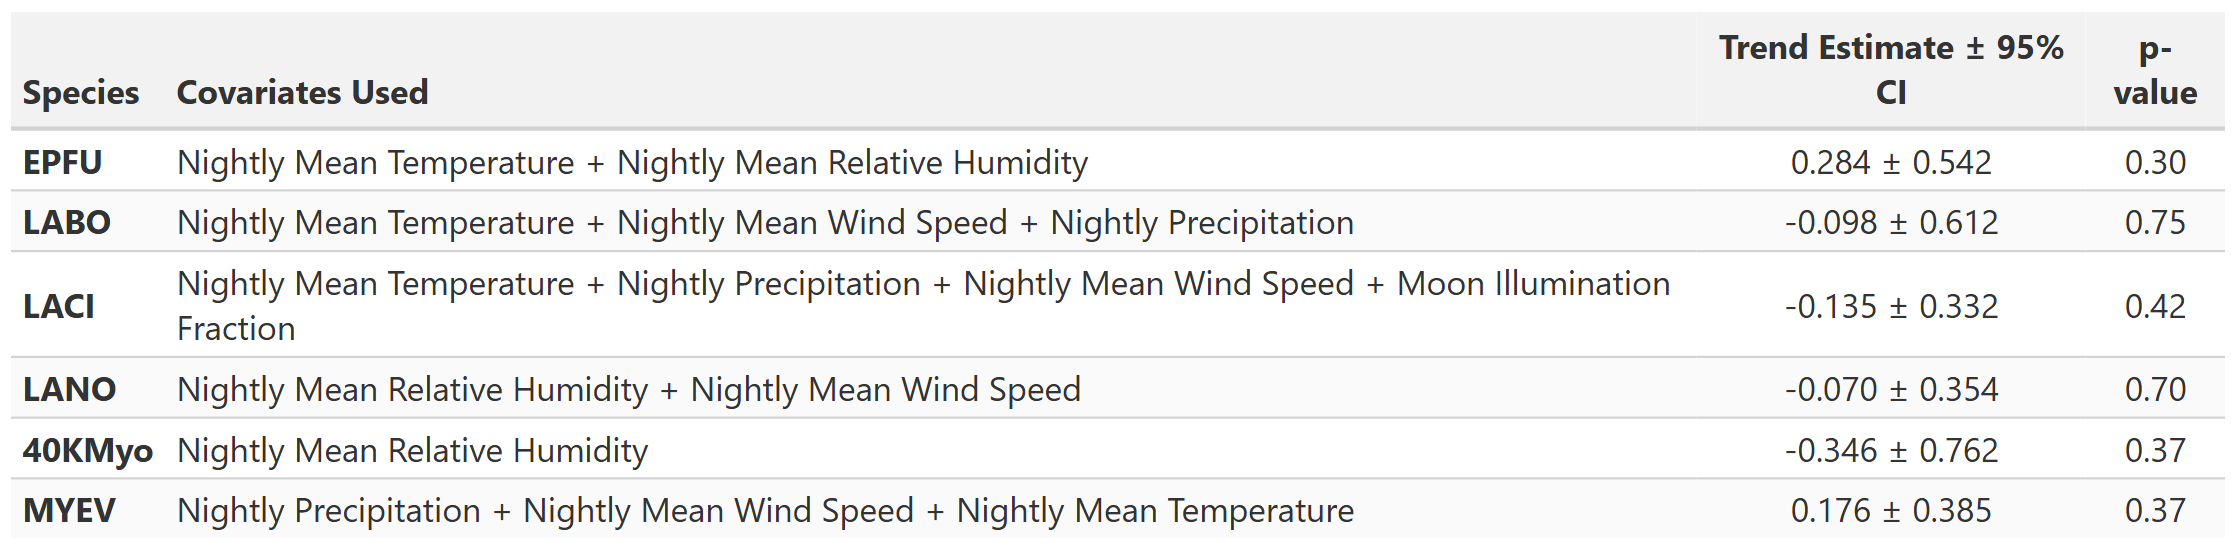
\includegraphics[width=7.46in,height=\textheight,keepaspectratio]{Figures/Trends/trend_table.png}

}

\end{table}%

\begin{figure}

\centering{

\pandocbounded{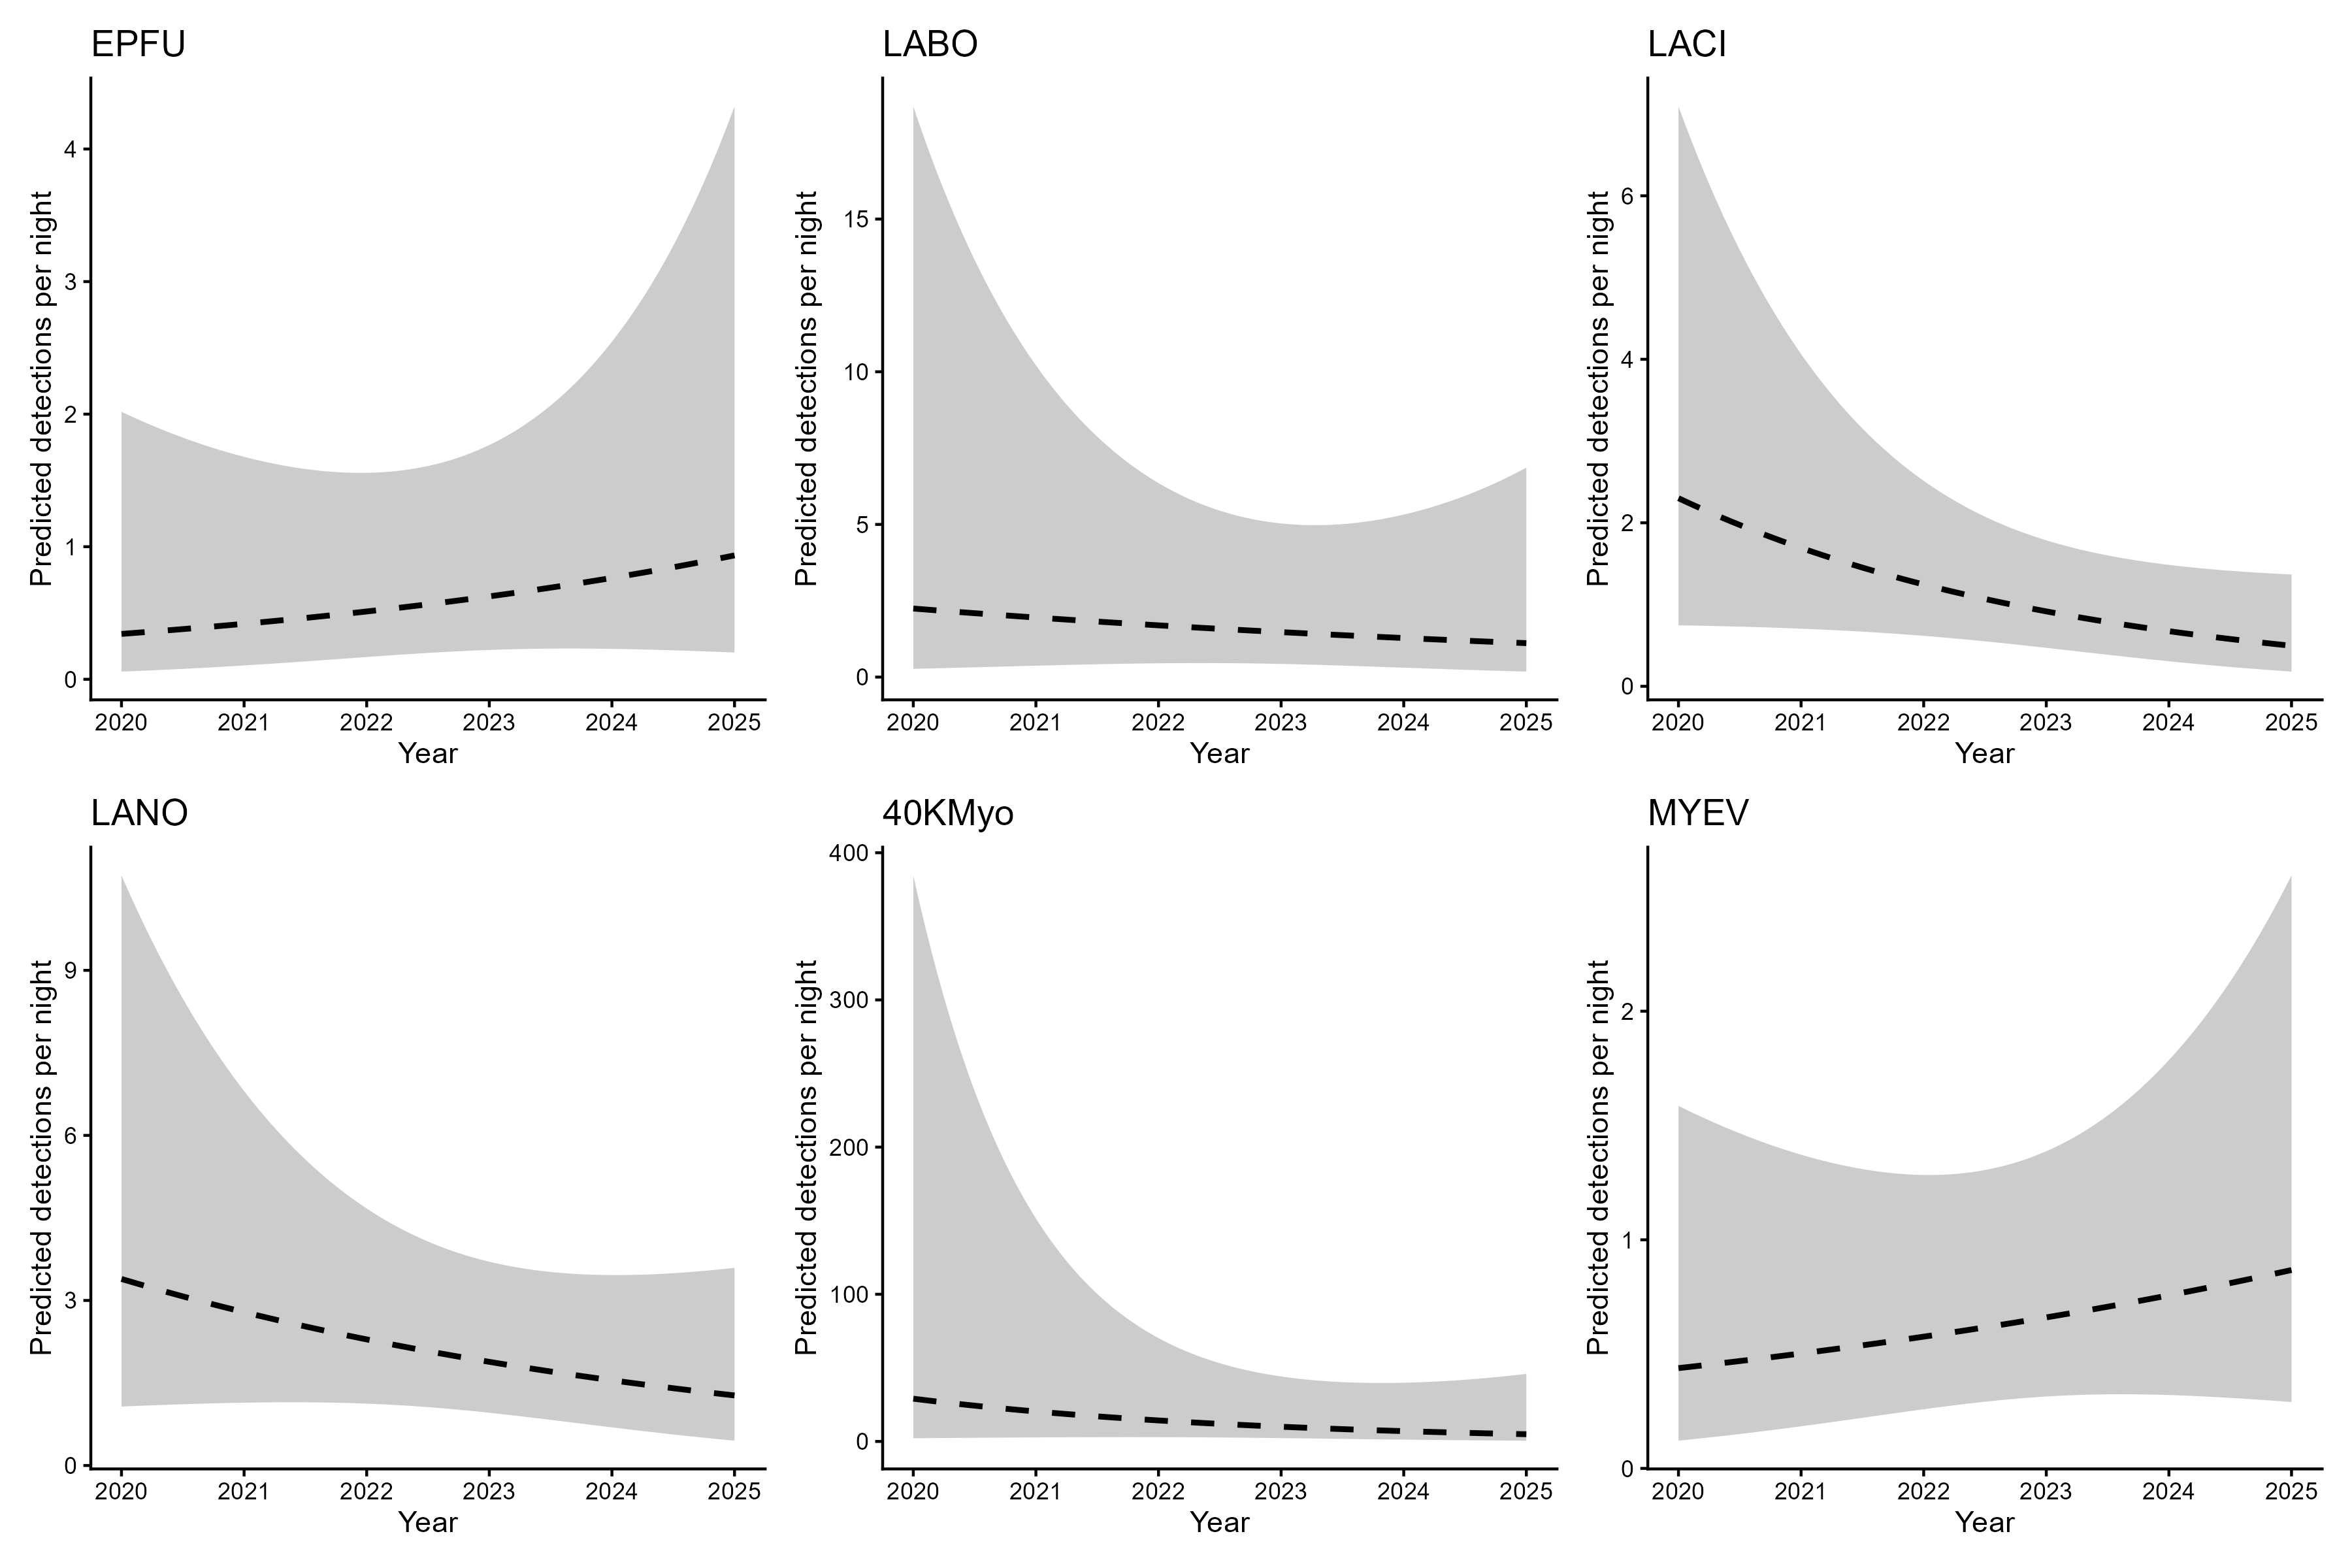
\includegraphics[keepaspectratio]{Figures/Trends/bat_trends_multipanel-det.png}}

}

\caption{\label{fig-trends}Species relative activity trends from
2020--2025 in the Banff NABat grid cell. Lines show trend estimates of
nightly detections with 95\% confidence intervals. Dashed lines indicate
non-significant trends (p \textgreater{} 0.05). Models are based on
nightly acoustic detections and fitted using negative binomial
mixed-effects models.}

\end{figure}%

\section{Discussion}\label{discussion}

Data used for trends only uses autoID from Kaleidoscope, which has been
shown to confuse Myotis spp. for LABO. so be careful here.

Results must be taken with caution because of small sample size, but
overall can conclude that bat species at the grid cell are stable. LACI
was almost significatna dn showed a decline, this means that close
inspection should be followed here. This is no suprise seeing the
increasing wind turbine development in the province and elsewhere.

How does this compare to the NABat abundance results for LABO, LACI and
LANO in the whole region?

Keep in mind that in the winter of 2026 WNS has been confirmed across
the Rockies and most importantly in Cadamun cave. This just points to
the importance of continues monitoring in the region. This will likely
be important to keep in mind and will mean the decrease of MYLU and MYSE

\section{Acknowledgements}\label{acknowledgements}

\newpage{}

\section{Appendix A}\label{appendix-a}

Species codes and their definitions

\begingroup\fontsize{9}{11}\selectfont

\begin{longtable*}{>{\raggedright\arraybackslash}p{3.5cm}>{\raggedright\arraybackslash}p{3.5cm}>{\raggedright\arraybackslash}p{2cm}>{\raggedright\arraybackslash}p{6cm}}
\toprule
CommonName & ScientificName & Code & Definition\\
\midrule
\endfirsthead
\multicolumn{4}{@{}l}{\textit{(continued)}}\\
\toprule
CommonName & ScientificName & Code & Definition\\
\midrule
\endhead

\endfoot
\bottomrule
\endlastfoot
\cellcolor{gray!10}{Big Brown Bat} & \cellcolor{gray!10}{Eptesicus fuscus} & \cellcolor{gray!10}{EPFU} & \cellcolor{gray!10}{Calls that have diagnostic features identifying it as Eptesicus fuscus}\\
Big Brown Bat / Silver-haired Bat & Eptesicus fuscus / Lasionycteris noctivagans & EPFULANO & Calls that could be attributed to either Eptesicus fuscus or Lasionycteris noctivagans\\
\cellcolor{gray!10}{Eastern Red Bat} & \cellcolor{gray!10}{Lasiurus borealis} & \cellcolor{gray!10}{LABO} & \cellcolor{gray!10}{Calls that have diagnostic features identifying it as Lasiurus borealis}\\
Eastern Red Bat / Little Brown Myotis & Lasiurus borealis / Myotis lucifugus & LABOMYLU & Calls that could be attributed to either Lasiurus borealis or Myotis lucifugus\\
\cellcolor{gray!10}{Hoary Bat} & \cellcolor{gray!10}{Lasiurus cinereus} & \cellcolor{gray!10}{LACI} & \cellcolor{gray!10}{Calls that have diagnostic features identifying it as Lasiurus cinereus}\\
\addlinespace
Hoary Bat / Silver-haired Bat & Lasiurus cinereus / Lasionycteris noctivagans & LACILANO & Calls that could be attributed to either Lasiurus cinereus or Lasionycteris noctivagans\\
\cellcolor{gray!10}{Silver-haired Bat} & \cellcolor{gray!10}{Lasionycteris noctivagans} & \cellcolor{gray!10}{LANO} & \cellcolor{gray!10}{Calls that have diagnostic features identifying it as Lasionycteris noctivagans}\\
Little Brown Myotis & Myotis lucifugus & MYLU & Calls that have diagnostic features identifying it as Myotis lucifugus\\
\cellcolor{gray!10}{Little Brown Myotis / Northern Myotis} & \cellcolor{gray!10}{Myotis lucifugus / Myotis septentrionalis} & \cellcolor{gray!10}{MYLUMYSE} & \cellcolor{gray!10}{Calls that could be attributed to either Myotis lucifugus or Myotis septentrionalis}\\
Northern Myotis & Myotis septentrionalis & MYSE & Calls that have diagnostic features identifying it as Myotis septentrionalis\\
\addlinespace
\cellcolor{gray!10}{40kHz Frequency Myotis} & \cellcolor{gray!10}{} & \cellcolor{gray!10}{40kMyo} & \cellcolor{gray!10}{Various species of Myotis that have a characteristic frequency in the range of 35-40kHz}\\
High Frequency Bat &  & HIGH FREQUENCY & Various species with pulses having a characteristic frequency higher than \textasciitilde{}35kHz\\
\cellcolor{gray!10}{Low Frequency Bat} & \cellcolor{gray!10}{} & \cellcolor{gray!10}{LOW FREQUENCY} & \cellcolor{gray!10}{Various species with pulses having a characteristic frequency lower than \textasciitilde{}30kHz}\\
Unknown Bat &  & NoID & Bat calls but no grouping category applies\\
\cellcolor{gray!10}{Noise} & \cellcolor{gray!10}{} & \cellcolor{gray!10}{Noise} & \cellcolor{gray!10}{No bat recorded}\\*
\end{longtable*}
\endgroup{}

\newpage{}

\section{Appendix B}\label{appendix-b}

Species detection summaries for each monitoring site.

\subsubsection*{Fenlands}\label{fenlands}

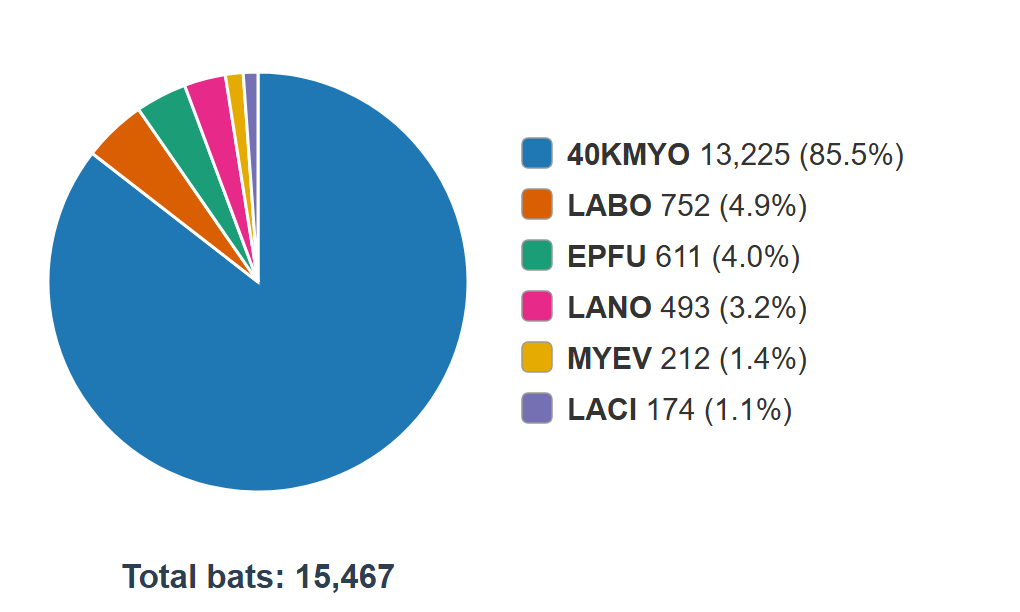
\includegraphics[width=0.6\linewidth,height=\textheight,keepaspectratio]{Figures/AppendixB/Fenlands_pie.png}

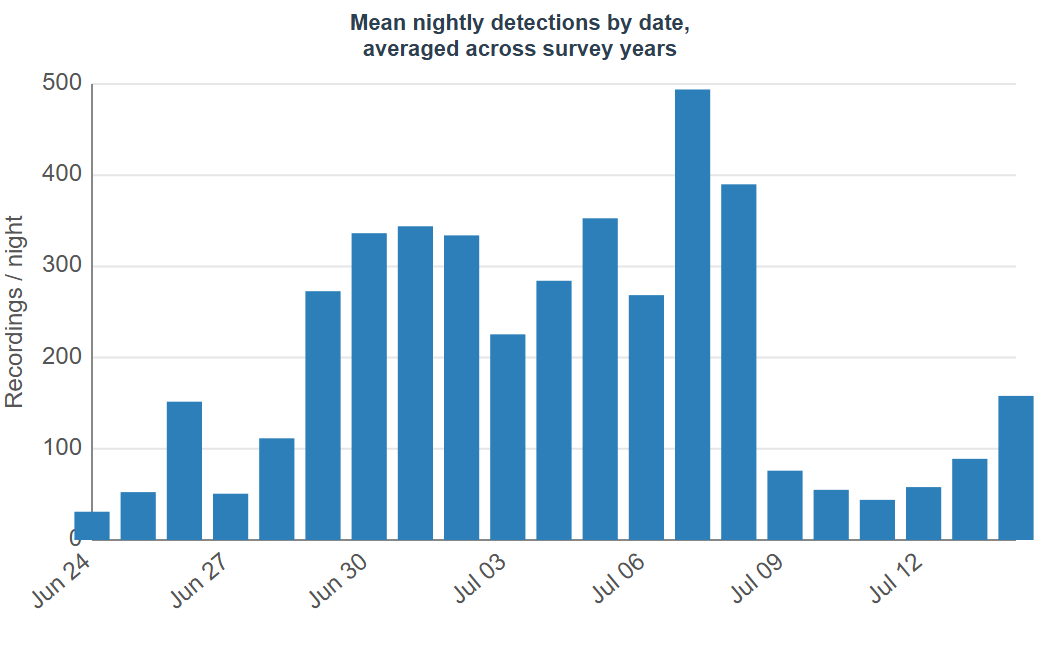
\includegraphics[width=0.6\linewidth,height=\textheight,keepaspectratio]{Figures/AppendixB/Fenlands_chart.png}

\newpage

\subsubsection*{Golf Course}\label{golf-course}

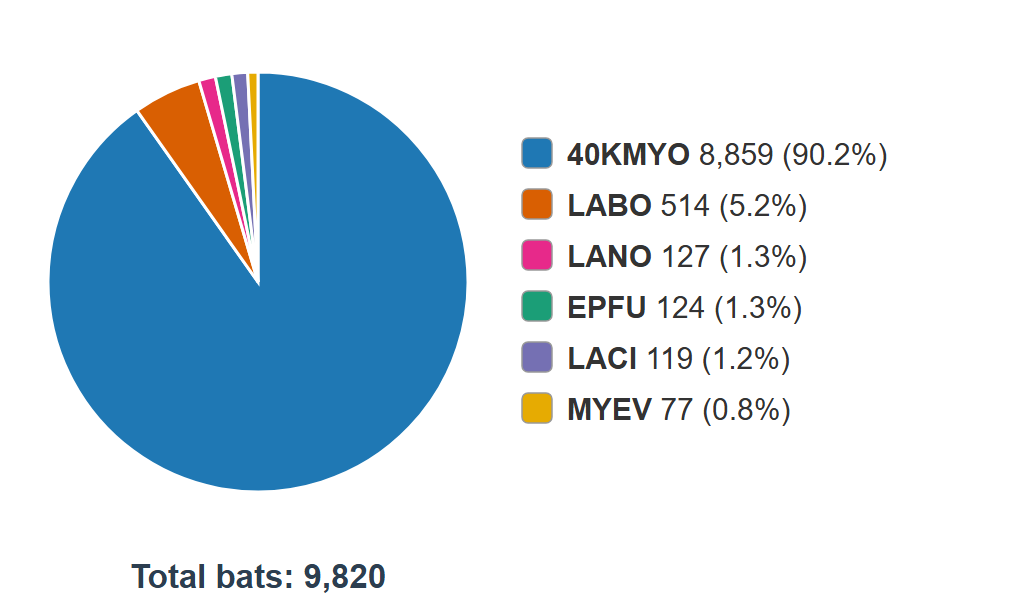
\includegraphics[width=0.6\linewidth,height=\textheight,keepaspectratio]{Figures/AppendixB/Golf_Course_pie.png}

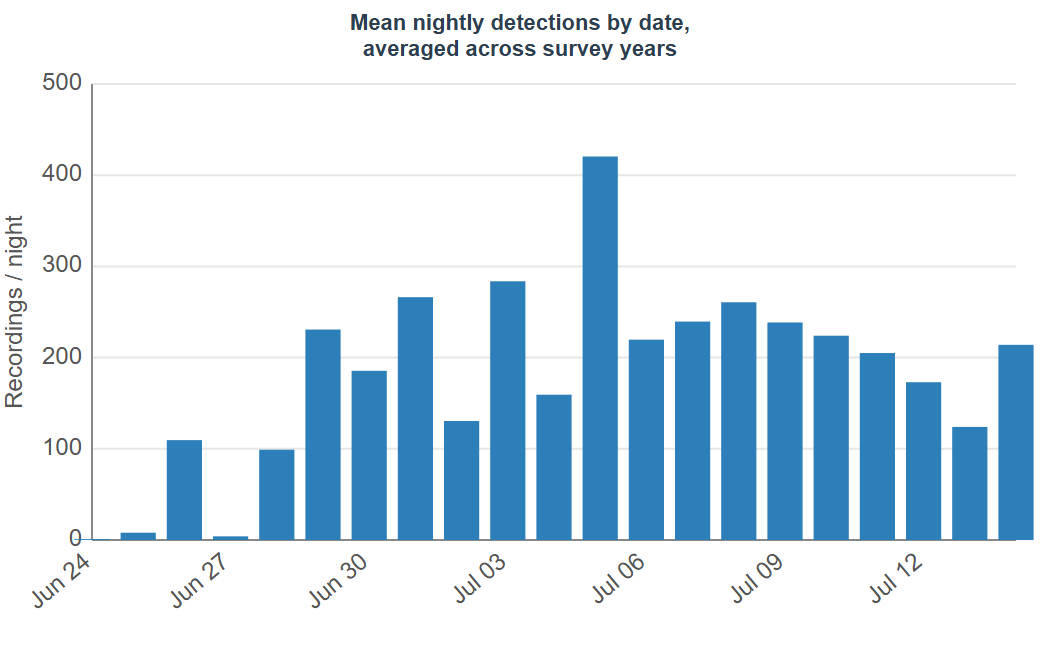
\includegraphics[width=0.6\linewidth,height=\textheight,keepaspectratio]{Figures/AppendixB/Golf_Course_chart.png}

\newpage

\subsubsection*{Upper Hotsprings}\label{upper-hotsprings}

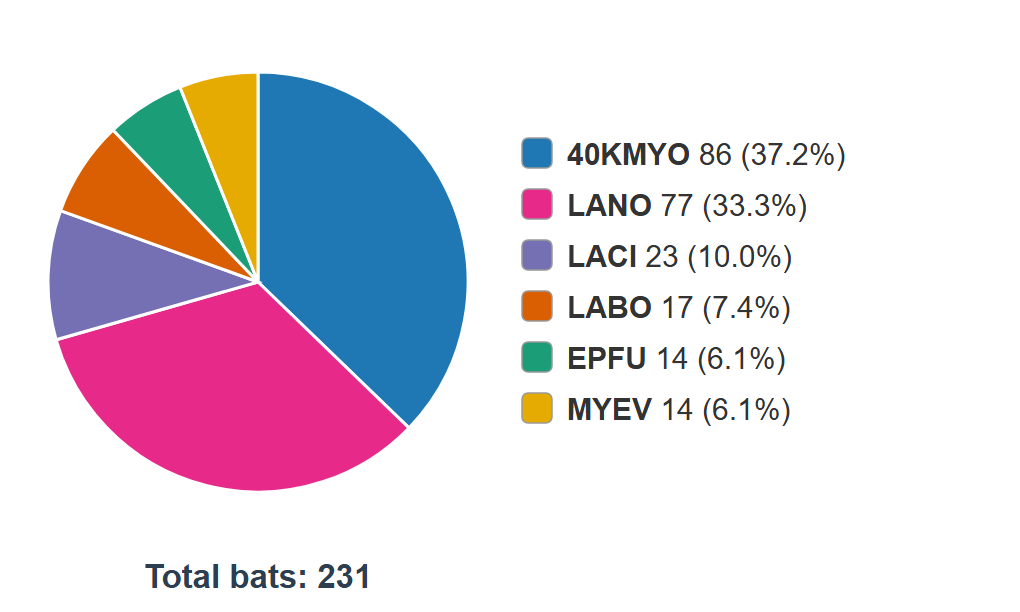
\includegraphics[width=0.6\linewidth,height=\textheight,keepaspectratio]{Figures/AppendixB/Upper_Hotsprings_pie.png}

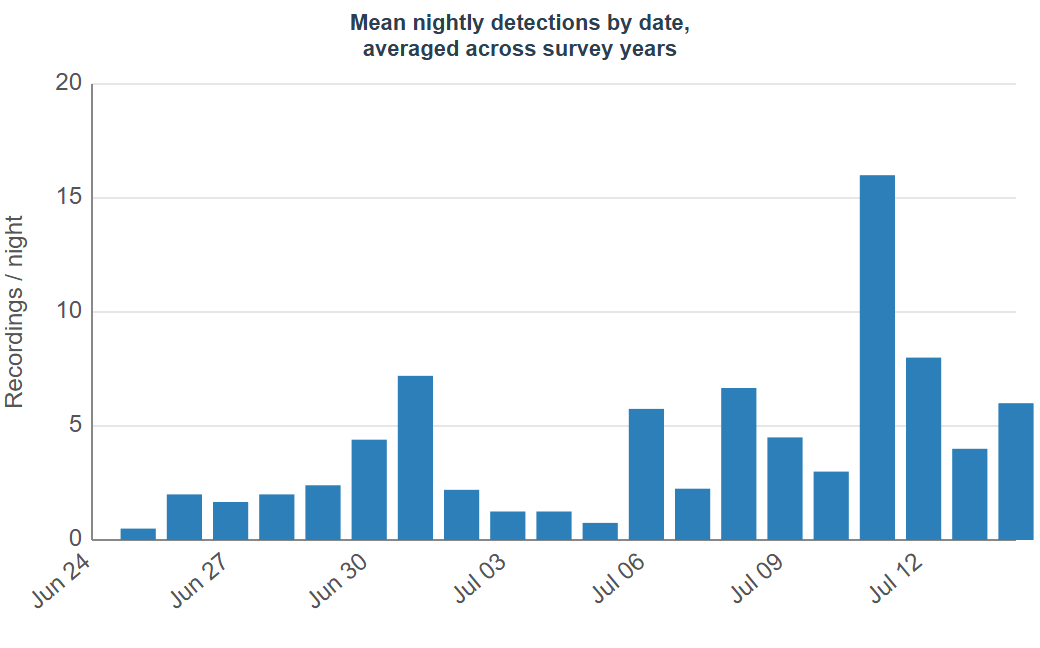
\includegraphics[width=0.6\linewidth,height=\textheight,keepaspectratio]{Figures/AppendixB/Upper_Hotsprings_chart.png}

\newpage

\subsubsection*{Driving Transect}\label{driving-transect}

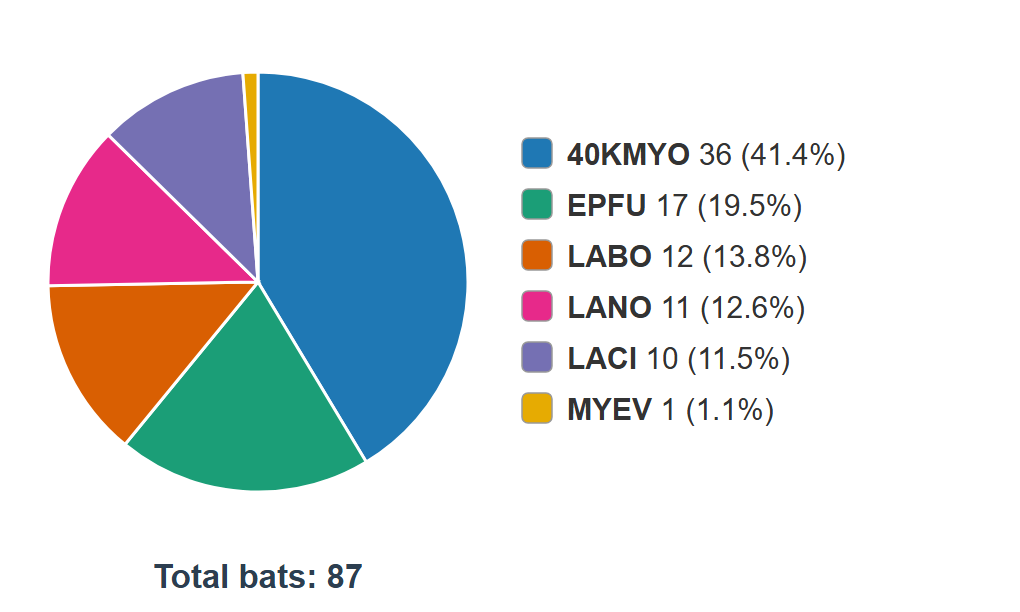
\includegraphics[width=0.6\linewidth,height=\textheight,keepaspectratio]{Figures/AppendixB/Driving_Transect_pie.png}

\newpage{}

\section*{Literature Cited}\label{literature-cited}
\addcontentsline{toc}{section}{Literature Cited}

\protect\phantomsection\label{refs}
\begin{CSLReferences}{1}{1}
\bibitem[\citeproctext]{ref-NRCan2025Wind}
{``Canadian Wind Turbine Database.''} 2025. Natural Resources Canada,
November 28.
\url{https://search.open.canada.ca/openmap/79fdad93-9025-49ad-ba16-c26d718cc070}.

\bibitem[\citeproctext]{ref-cwhc-rcsf2024Canadian}
CWHC-RCSF. 2024. {``Canadian {Wildlife Health Cooperative} - {Réseau}
Canadien Pour La Santé de La Faune.''}
\url{https://www.cwhc-rcsf.ca/white_nose_syndrome_reports_and_maps.php}.

\bibitem[\citeproctext]{ref-ministryofenergyandclimatesolutions2024BC}
Energy and Climate Solutions, Ministry of. 2024. {``{BC Gov News}.''}
December 9. \url{https://news.gov.bc.ca/releases/2024ECS0048-001643}.

\bibitem[\citeproctext]{ref-friedenberg2021Assessing}
Friedenberg, Nicholas A., and Winifred F. Frick. 2021. {``Assessing
Fatality Minimization for Hoary Bats Amid Continued Wind Energy
Development.''} \emph{Biological Conservation} 262 (October): 109309.
\url{https://doi.org/10.1016/j.biocon.2021.109309}.

\bibitem[\citeproctext]{ref-loeb2015Plan}
Loeb, Susan C., Thomas J. Rodhouse, Laura E. Ellison, et al. 2015.
\emph{A Plan for the {North American Bat Monitoring Program} ({NABat})}.
SRS-GTR-208. U.S. Department of Agriculture, Forest Service, Southern
Research Station. \url{https://doi.org/10.2737/SRS-GTR-208}.

\bibitem[\citeproctext]{ref-olsonBat}
Olson, Cory. n.d. {``Bat {Profiles}.''} Alberta Community Bat Program.
Accessed March 6, 2025. \url{https://www.albertabats.ca/batprofiles/}.

\bibitem[\citeproctext]{ref-rae2022North}
Rae, Jason, and Cori L Lausen. 2022. \emph{North {American Bat
Monitoring Program} in {British Columbia}: 2021 {Data Summary} and
{Activity Trend Analyses} (2016-2021).} Wildlife Conservation Society of
Canada.

\bibitem[\citeproctext]{ref-rae2024North}
Rae, Jason, and Cori L Lausen. 2024. \emph{North {American Bat
Monitoring Program} in {British Columbia}: 2023 {Data Summary} and
{Activity Trend Analyses} (2016-2023).} Wildlife Conservation Society of
Canada.

\bibitem[\citeproctext]{ref-reichert2018}
Reichert, Brian, Cori Lausen, Susan Loeb, et al. 2018a. \emph{A Guide to
Processing Bat Acoustic Data for the North American Bat Monitoring
Program (NABat)}.

\bibitem[\citeproctext]{ref-reichert2018Guide}
Reichert, Brian, Cori Lausen, Susan Loeb, et al. 2018b. \emph{A {Guide}
to {Processing Bat Acoustic Data} for the {North American Bat Monitoring
Program} ({NABat})}. Open-File Nos. 2018--1068. U.S. Geological Survey.

\bibitem[\citeproctext]{ref-slough2022New}
Slough, Brian, Cori Lausen, Brian Paterson, et al. 2022. {``New Records
about the Diversity, Distribution, and Seasonal Activity Patterns by
Bats in {Yukon} and Northwestern {British Columbia}.''}
\emph{Northwestern Naturalist} 103 (August): 162--82.
\url{https://doi.org/10.1898/NWN21-10}.

\bibitem[\citeproctext]{ref-solick2022Bat}
Solick, Donald. 2022. {``Bat {Acoustic Species-Pair Matrix Western
US}/{Canada}.''}
\url{https://www.batacousticsurveys.com/_files/ugd/a1e0ca_0ed9c3172b9145e49c50eb7a7712f909.pdf}.

\bibitem[\citeproctext]{ref-committeeonthestatusofendangeredwildlifeincanada2023Hoary}
Status of Endangered Wildlife in Canada, Committee on the. 2023.
{``Hoary {Bat} ({Lasiurus} Cinereus) {Eastern Red Bat} ({Lasiurus}
Borealis) {Silver-haired Bat} ({Lasionycteris} Noctivagans): {COSEWIC}
Assessment and Status Report 2023.''}
\url{https://www.canada.ca/en/environment-climate-change/services/species-risk-public-registry/cosewic-assessments-status-reports/hoary-bat-eastern-red-bat-silver-haired-bat-2023.html}.

\bibitem[\citeproctext]{ref-stratton2022Coupling}
Stratton, Christian, Kathryn M. Irvine, Katharine M. Banner, Wilson J.
Wright, Cori Lausen, and Jason Rae. 2022. {``Coupling Validation Effort
with in Situ Bioacoustic Data Improves Estimating Relative Activity and
Occupancy for Multiple Species with Cross‐species Misclassifications.''}
\emph{Methods in Ecology and Evolution} 13 (6): 1288--303.
\url{https://doi.org/10.1111/2041-210X.13831}.

\bibitem[\citeproctext]{ref-szewczak2018Acoustic}
Szewczak, Joe. 2018. \emph{Acoustic {Features} of {Western US Bats}}.
Humboldt State University Bat Lab.

\bibitem[\citeproctext]{ref-u.s.fishandwidlifeserviceusfws2025WhiteNose}
USFWS, U. S. Fish and Widlife Service. 2025. {``White-{Nose
Syndrome}.''} \url{https://www.whitenosesyndrome.org/}.

\bibitem[\citeproctext]{ref-zimmerling2016Bat}
Zimmerling, J. Ryan, and Charles M. Francis. 2016. {``Bat Mortality Due
to Wind Turbines in {Canada}.''} \emph{The Journal of Wildlife
Management} 80 (8): 1360--69. \url{https://doi.org/10.1002/jwmg.21128}.

\end{CSLReferences}




\end{document}
